\documentclass[pdflatex,Numbered]{sn-jnl}

% ---------- Packages ----------
\usepackage{graphicx}%
\usepackage{multirow}%
\usepackage{amsmath,amssymb,amsfonts}%
\usepackage{amsthm}%
\usepackage{mathrsfs}%
\usepackage[title]{appendix}%
\usepackage{xcolor}%
\usepackage{textcomp}%
\usepackage{manyfoot}%
\usepackage{booktabs}%
\usepackage{algorithm}%
\usepackage{algorithmicx}%
\usepackage{algpseudocode}%
\usepackage{listings}%
\usepackage{array}%
\usepackage{tabularx}%
\usepackage{caption}%
\usepackage{subcaption}%
\usepackage{makecell}%
\usepackage{float}% provides [H] for exact float placement
\usepackage[section]{placeins}% auto-FloatBarrier at section breaks
\usepackage[numbers,sort&compress]{natbib}%
\usepackage{hyperref}%

\theoremstyle{plain}
\newtheorem{theorem}{Theorem}
\newcommand{\fallback}{\textit{not clearly stated in the retrieved evidence}}

% ---------- Title ----------
\title[Structural safety in patient-facing onboarding AI]{Structural Safety in Patient-Facing AI for Clinical Trial Onboarding: An Audited Grounded Pipeline}

\author[1]{\fnm{Md Zabirul} \sur{Islam}}\email{islamm11@rpi.edu}
\author*[2]{\fnm{Ge} \sur{Wang}}\email{wangg6@rpi.edu}

\affil[1]{\orgdiv{Department of Computer Science}, \orgname{Rensselaer Polytechnic Institute}, \orgaddress{\city{Troy}, \state{NY}, \country{USA}}}
\affil[2]{\orgdiv{Department of Biomedical Engineering}, \orgname{Rensselaer Polytechnic Institute}, \orgaddress{\city{Troy}, \state{NY}, \country{USA}}}


\abstract{\textbf{Background.} Patient-facing artificial intelligence (AI) systems for clinical trial onboarding may improve access to study information, but they also introduce a specific safety risk: \emph{cross-trial conflation}, in which a single response combines eligibility criteria, procedures, or time commitments from different trials. Existing trial-matching systems typically optimize patient--trial matching accuracy and do not explicitly enforce single-trial consistency across patient-facing outputs.

\textbf{Methods.} We developed a grounded onboarding pipeline in which a five-gate selector either accepts one dominant trial as the evidence source or abstains with a patient-facing clarification prompt. Eligibility triage, consent-style explanation, and teach-back generation are then constrained to the accepted trial. We evaluated the pipeline on 114 cases across six therapeutic areas and two selector regimes. Six model families produced 684 generations under identical guarded conditions. Outputs were audited using three pre-specified leak detectors: two deterministic lexical detectors and one semantic auditor based on two independent large language model (LLM) judges, and blind-scored by two LLM judges using a five-dimension rubric. We further contrasted the pipeline against four pre-registered evidence-control baselines (standard multi-trial retrieval-augmented generation, prompt-only guarding, citation-enforced generation, and trivial top-1 selection; 912 additional generations), classified flagged generations into a three-way failure taxonomy, and implemented a claim-level natural-language-inference (NLI) verifier for the residual semantic channel.

\textbf{Results.} The lexical detectors flagged $0/684$ generations, corresponding to Clopper--Pearson upper 95\% bounds of $0.54\%$ pooled and $3.2\%$ stem-clustered. The semantic auditor flagged $12/684$ generations ($1.75\%$) under both-judges-agree consensus (Cohen's $\kappa = 0.16$; raw agreement, $86.5\%$). Manual review classified eight of these cases as paraphrased cross-trial content, two as mixed-attribution errors, and two as likely judge over-flags. Semantic leakage was concentrated in the structurally adversarial subset, defined by dominance ratio $\rho < 1.5$ and at least two trials in the candidate pool, and was highest for the smallest backbone. Qwen-2.5-7B achieved the highest overall rubric score ($3.95/5$; 95\% confidence interval, $3.76$--$4.14$). The lower-latency Qwen-2.5-3B candidate preserved high safety scores while reducing mean latency by $44\%$ ($11.0$ vs.\ $19.8$ s). Inter-judge agreement was moderate on substantive rubric dimensions (Spearman $r_s = 0.52$--$0.56$). The selector score share showed negative Brier skill and should not be interpreted as a calibrated triage probability. The baseline contrast was decisive: standard multi-trial RAG, prompt-only guarding, and citation enforcement leaked under the dual-judge semantic consensus at $50.9$--$59.0\%$ (predominantly cross-trial contamination), whereas the two structural single-trial systems---trivial top-1 selection and the deployed pipeline---held semantic-consensus leakage at $1.3\%$ and $1.8\%$ with zero contamination-class failures, and top-1 selection simultaneously attained the highest baseline utility. A claim-level NLI verifier removed $8$ of the $12$ consensus semantic leaks (exactly those manual review deemed genuine cross-trial content) at a $15.1\%$ per-claim utility cost.

\textbf{Conclusions.} Cross-trial conflation can be reduced by enforcing single-trial evidence control before generation rather than relying only on the generator; the baseline comparison shows that only structural single-trial control closes the channel, while prompt-only and citation-based mitigations do not. In this audited cohort, no lexical cross-trial leakage was detected, while a smaller semantic paraphrase channel persisted, was empirically bounded, and was further reduced by claim-level NLI verification. The proposed pipeline is end-to-end auditable and produces either a coordinator-reviewable pre-screening bundle or a clarification prompt, rather than issuing eligibility verdicts directly to patients.}

\keywords{clinical trial onboarding, patient-facing artificial intelligence, cross-trial leakage, informed consent, teach-back, safety-first artificial intelligence}


\begin{document}
\maketitle

% ============================================================

\section{Introduction}

Clinical trial participation remains limited by trial availability and by patients' ability to determine whether a study may be relevant to them; recruitment shortfalls and uneven access disproportionately affect minoritized populations and rural patients \citep{unger2019recruitment,clark2019barriers,fda2022diversity}. Eligibility criteria are usually written in formal protocol language, whereas patient questions are often expressed in lay terms. Patient-facing AI systems may help bridge this communication gap, but they also create safety risks when generated responses are not strictly grounded. LLMs can produce fluent but inaccurate medical content \citep{ji2023hallucination,maynez2020faithfulness,pal2023medhalu,huang2025survey,ayers2023comparing}, and this risk is amplified when responses are read directly by patients rather than reviewed first by clinicians or study coordinators.

The safety problem targeted in this study is \emph{cross-trial conflation}: a patient-facing response that combines information from multiple clinical trials, such as eligibility criteria from one trial, procedures from another, and time commitments from a third. This failure mode is distinct from isolated hallucination because each individual statement may resemble real trial content, while the combined response no longer describes any single protocol. The downstream consequences are clinically meaningful. A patient may form an incorrect belief about eligibility, self-exclude from a trial for which they might qualify, arrive at screening with expectations based on another protocol's procedures or schedule, or lose trust in the recruiting institution when the discrepancy is discovered. Each such case may also require additional coordinator time to identify and correct the error.

Existing AI-assisted trial-matching systems, including DeepEnroll \citep{zhang2020deepenroll}, COMPOSE \citep{gao2020compose}, TrialGPT \citep{jin2024trialgpt}, PRISM \citep{gupta2024prism}, Trial2Vec \citep{wang2023trial2vec}, criterion-vector eligibility ranking \citep{bustos2018trial}, and recent oncology-scale work \citep{wong2024scaling,nievas2024distilling,chen2025enhancing}, primarily optimize criterion-level or patient--trial matching accuracy. These systems produce an eligibility assessment for a given patient--trial pair, but they do not explicitly enforce single-trial consistency across the multiple outputs required in an onboarding interaction. Patient-facing LLM wrappers, including medical-domain models such as Med-PaLM and its successors \citep{singhal2023medpalm,singhal2025medpalm2,lievin2024can}, inherit the same limitation. Retrieval-augmented generation \citep{lewis2020rag,karpukhin2020dpr,thakur2021beir,zhao2025medrag,xiong2024benchmarking,neha2025ragsystematic} supplies external evidence, but the generator may still combine information from multiple trials when the retrieved evidence pool spans more than one protocol. Clinical foundation-model deployment also remains sensitive to grounding failures and distribution shift \citep{wornow2023shaky,topol2019deep,obermeyer2019dissecting}.

To our knowledge, prior trial-matching evaluations have not reported a cross-trial leak rate. This gap arises because the dominant evaluation unit is the patient--trial pair, whereas cross-trial conflation is an interaction-level consistency failure. A single patient-facing response that mixes content from two or more trials is not directly captured by per-pair training objectives or evaluation metrics. We therefore evaluate cross-trial conflation as a patient-facing safety dimension for clinical trial onboarding.



We address cross-trial conflation at the evidence layer. The proposed grounded onboarding pipeline (Fig.~\ref{fig:pipeline}) uses a five-gate trial-first selector that either accepts a single dominant trial as the unique evidence context or abstains with a patient-facing clarification prompt. Downstream modules for eligibility triage, consent-style explanation with evidence-bounded fallback, and uncertainty-aware teach-back all draw from the accepted trial. Each patient-facing output is either traceable to a cited passage from that trial or replaced by an explicit fallback statement.

This work is framed as an early-stage clinical-AI safety study \citep{vasey2022decideai}. Reporting is guided by the CLAIM checklist for clinical AI \citep{mongan2020claim}, TRIPOD+AI guidance for prediction-model reporting \citep{collins2024tripodai}, and CONSORT-AI/SPIRIT-AI extensions for AI interventions in clinical workflows \citep{liu2020spiritai}. If adapted for clinical use, the system would require prospective evaluation under applicable software as a medical device (SaMD) and clinical-AI governance frameworks, including guidance from the U.S. Food and Drug Administration (FDA) on AI/ML-based SaMD \citep{fda2021samdaction}, the European Medicines Agency (EMA) reflection paper on AI in the medicines lifecycle \citep{ema2024reflection}, and the World Health Organization (WHO) guidance on large multimodal models in health \citep{who2024llm}. Consistent with critiques of post-hoc explainability in clinical AI \citep{ghassemi2021falsehope}, our focus is not model-internal explanation but structural audit traceability: patient-facing claims must be linked to accepted evidence or replaced by fallback text.

We make four contributions:

\begin{enumerate}
\item \textbf{An empirical safety evaluation within an audited regime} (\S\ref{sec:results_leak}--\S\ref{sec:results_pergate}). Across 684 generations from six model families, six therapeutic areas, two selector regimes, and five leave-one-out per-gate ablations, two deterministic lexical detectors identified no cross-trial leakage. These detectors included a narrow ClinicalTrials.gov \texttt{NCT} identifier detector and a wider entity-resolved detector. We report this as an empirical bound under correlated samples, not as an absolute guarantee (Clopper--Pearson upper 95\% bounds: $0.54\%$ pooled and $3.2\%$ stem-clustered). A third semantic LLM-judge detector identified $12/684$ generations ($1.75\%$) under both-judges-agree consensus (Cohen's $\kappa = 0.16$). Manual review classified $8/12$ as paraphrased cross-trial content, $2/12$ as mixed-attribution errors, and $2/12$ as likely judge over-interpretation of generic clinical language. These semantic cases were not detectable by lexical methods and were concentrated in structurally adversarial cases (dominance ratio $<1.5$ with $\geq 2$ candidate trials; \S\ref{sec:results_adversarial}).

\item \textbf{A backbone-invariance analysis for the lexical leak channel} (\S\ref{sec:results_backbone_gate}--\S\ref{sec:results_abstain}). The zero-lexical-leak result held across four open-weight and two closed application programming interface (API) generators, while valid-parse, commit, and fluency-related behavior varied substantially. This invariance applies to the lexical safety axis, not to overall utility. Weaker backbones may remain safe by abstaining or returning schema-default fallback text, whereas stronger backbones produce more useful committed outputs. The safety mechanism is therefore located primarily in the selector and post-processor rather than in any single generator backbone.

\item \textbf{A deterministic sufficiency theorem with explicit boundary conditions} (Theorem~\ref{thm:safety}). We formalize three operational invariants: single-trial evidence, bounded fallback, and schema enforcement. Together, these invariants are sufficient for zero lexical leakage under schema-constrained outputs. We also specify the deployment conditions under which this bound would not apply, including the paraphrased semantic channel measured by the semantic auditor.

\item \textbf{An auditable clinical deployment-evaluation workflow} (Fig.~\ref{fig:deployment}). The proposed workflow defines roles for the patient, the pipeline, the study coordinator, and the audit/governance layer. For each query, the system persists an audit bundle containing the evidence set, selector decisions, raw and post-processed generations, blinded judge scores, per-gate ablations, and inter-rater reliability outputs. These artifacts are released to support reproduction, audit, and extension of the reported results.
\end{enumerate}

\begin{figure}[!htbp]
\centering
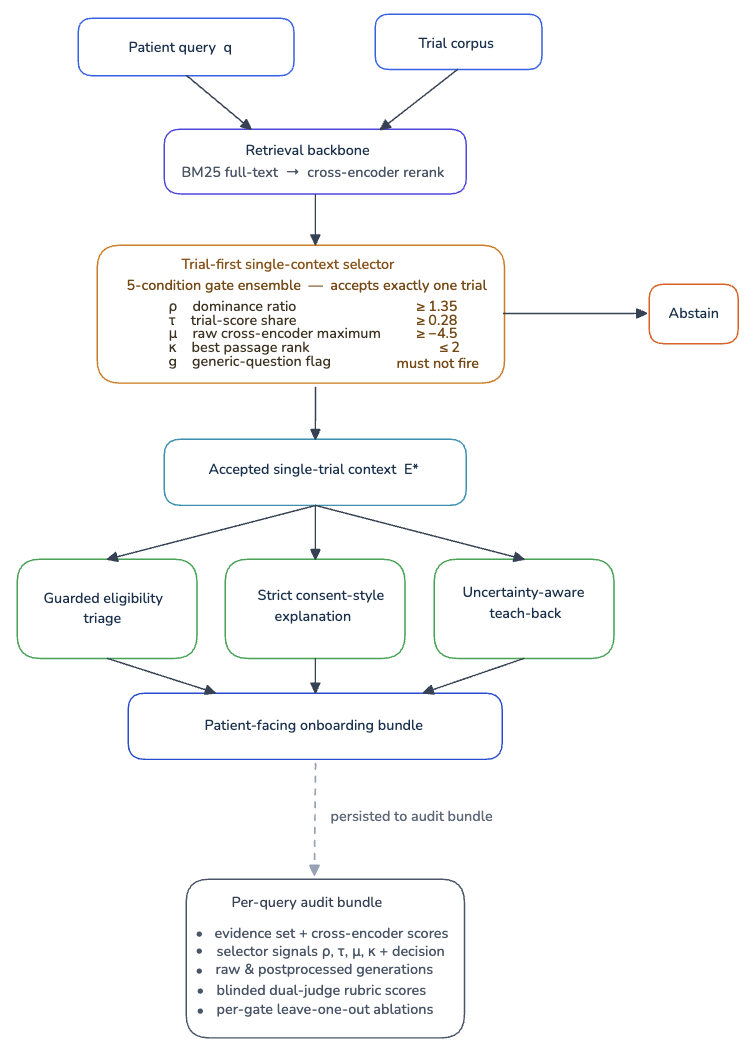
\includegraphics[width=0.96\linewidth]{figures/pipeline_architecture.png}
\caption{\textbf{Grounded clinical trial onboarding pipeline.} A patient query and the trial corpus enter the retrieval backbone (BM25 full-text retrieval followed by cross-encoder reranking). The trial-first selector accepts a single dominant trial only if its dominance ratio $\rho$, score share $\tau$, raw cross-encoder maximum $\mu$, and best rank $\kappa$ clear configured thresholds and the query is not flagged as generic. Otherwise, the pipeline abstains with a clarification prompt. Downstream modules for guarded eligibility triage, consent-style explanation with evidence-bounded fallback, and uncertainty-aware teach-back all draw from the same accepted trial. Audit artifacts are persisted for each query.}
\label{fig:pipeline}
\end{figure}



% ============================================================

\section{Results}
\label{sec:results}

\subsection{Zero detected lexical cross-trial leakage under the audited conditions; residual semantic leakage quantified}
\label{sec:results_leak}

Across 114 onboarding cases, six model families, two selector regimes, and two pre-specified \emph{lexical} leak definitions, the cross-trial leak rate was $0\%$ (Table~\ref{tab:six_backbone}; per-cell heatmap in Supplementary Information \S~5). The narrow definition flagged any \texttt{NCT} identifier other than the selected trial in any model-emitted text field. The wide definition additionally matched distinctive non-stop title tokens unique to a single non-selected trial. Both definitions produced the same result: $0/684$ generations.

Lexical detectors cannot capture paraphrased cross-trial content by construction. We therefore added a third pre-specified semantic detector. Each generation was independently scored by Claude Sonnet~4.5 and GPT-4o under a structured rubric that returned a binary \texttt{semantic\_leak} flag, the suspect non-selected trial, a verbatim claim excerpt of up to 250 characters, and a two-sentence rationale (prompt in Supplementary Information \S2.6). Across the 684-generation audit, the semantic detector flagged $12/684$ generations ($1.75\%$) under both-judges-agree consensus (Cohen's $\kappa = 0.16$; raw agreement, $86.5\%$; pooled either-judge rate, $104/684 = 15.2\%$). The low $\kappa$ despite high raw agreement reflects the rarity of consensus flags and the associated prevalence imbalance, as discussed in \S\ref{sec:results_irr_brief}.

Manual review of the 12 consensus-flagged cases classified eight as unambiguous paraphrased cross-trial content, two as mixed-attribution errors, and two as likely judge over-interpretation of generic clinical language that also fit the selected trial. Examples of unambiguous cases included a HER2-positive eligibility claim asserted for a HER2-negative selected trial, a one-year-post-pituitary-surgery exclusion attributed to a trial whose criteria did not contain that exclusion, and a continued-octreotide-LAR treatment plan asserted for a selected trial that described only surgical resection. The largest per-backbone semantic residual was observed for the smallest open-weight backbone, Qwen-2.5-3B ($3.51\%$), whereas the closed-API baselines had the lowest residual rate ($0.88\%$ each). All 12 consensus-flagged cases passed the lexical detectors, indicating that lexical and semantic detectors measured distinct leakage channels.

\begin{table}[!htbp]
\centering
\caption{\textbf{Six-backbone safety summary on the $n=114$ pool} ($684$ generations total). Closed-API baselines were evaluated zero-shot using the same guarded evidence and JSON-schema prompt; no fine-tuning was used. Lexical leak rate was zero for every model under both definitions. The rightmost column reports the semantic detector under both-judges-agree consensus. Leak$_{\mathrm{nar}}$: narrow \texttt{NCT}-identifier detector; Leak$_{\mathrm{wide}}$: wide entity-resolved detector; Leak$_{\mathrm{sem}}$: semantic dual-judge consensus. Qwen-2.5-3B is treated as a low-latency candidate backbone; the system is not clinically deployed.}
\label{tab:six_backbone}
\footnotesize
\setlength{\tabcolsep}{3pt}
\begin{tabular}{lcccccccc}
\toprule
Model & Family & $N$ & Parse-ok & Commit & Abstain & Leak$_{\mathrm{nar}}$ & Leak$_{\mathrm{wide}}$ & Leak$_{\mathrm{sem}}$ \\
\midrule
Qwen-2.5-3B          & open-weight & 114 & 0.63 & 0.55 & 0.00 & \textbf{0.00} & \textbf{0.00} & 0.035 \\
Qwen-2.5-7B          & open-weight & 114 & 0.89 & 0.44 & 0.00 & \textbf{0.00} & \textbf{0.00} & 0.018 \\
Meta-Llama-3.1-8B    & open-weight & 114 & 0.39 & 0.19 & 0.00 & \textbf{0.00} & \textbf{0.00} & 0.018 \\
Mistral-7B-v0.3      & open-weight & 114 & 0.12 & 0.11 & 0.01 & \textbf{0.00} & \textbf{0.00} & 0.018 \\
GPT-4o               & closed-API  & 114 & \textbf{1.00} & 0.31 & 0.04 & \textbf{0.00} & --- & \textbf{0.009} \\
Claude Sonnet~4.5    & closed-API  & 114 & \textbf{1.00} & 0.14 & 0.11 & \textbf{0.00} & --- & \textbf{0.009} \\
\bottomrule
\end{tabular}
\end{table}

The result was consistent across six therapeutic-area strata: musculoskeletal, cardiovascular, metabolic/endocrine, oncology, neurology/CNS, and a heterogeneous Other category (Fig.~\ref{fig:per_area}). Every one of the 24 area-by-open-weight-backbone cells had lexical leak rate $0$. Commit and parse-ok rates varied by backbone, consistent with the fluency and format-following differences shown in Table~\ref{tab:six_backbone}.

\begin{figure}[!htbp]
\centering
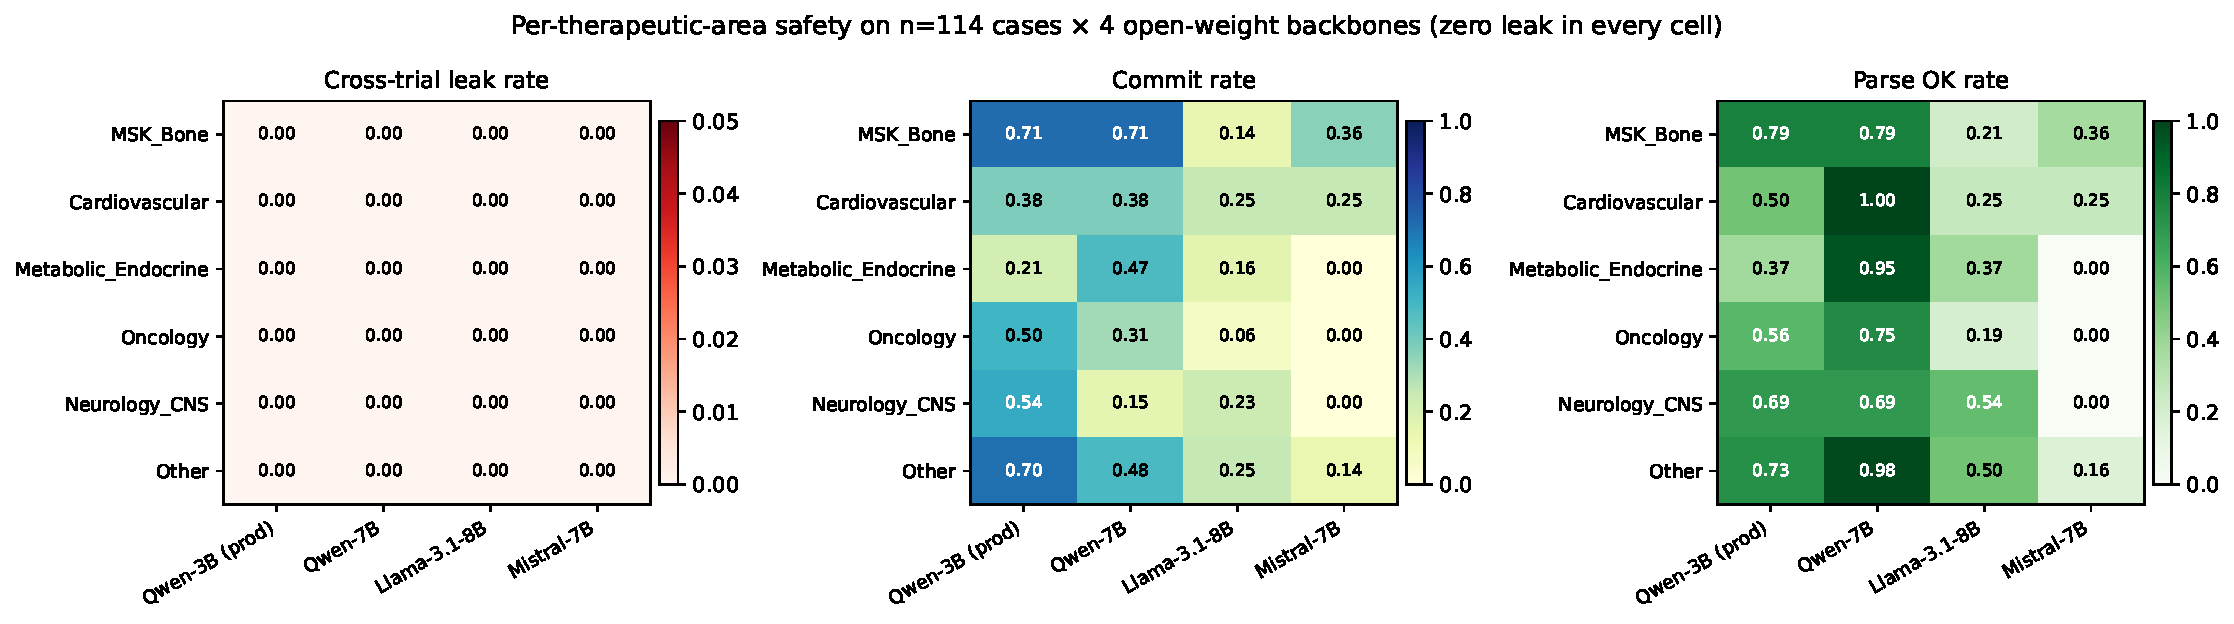
\includegraphics[width=0.96\linewidth]{figures/per_area_heatmap.pdf}
\caption{\textbf{Per-(therapeutic area $\times$ backbone) behavior on $n=114$ open-weight cases.} Left: cross-trial leak rate, which is $0$ in every cell. Center: commit rate. Right: parse-ok rate. Commit and parse-ok rates vary by backbone, whereas the lexical safety result is preserved across all six therapeutic areas tested.}
\label{fig:per_area}
\end{figure}

\subsection{Per-gate ablation shows that no single gate explains the zero-lexical-leak result}
\label{sec:results_pergate}

We next tested whether the zero-lexical-leak result depended on any single selector gate. In a leave-one-out counterfactual ablation, each gate was dropped while the others remained active (Methods, \S\ref{sec:methods_pergate}). Three variants admitted additional cases relative to the deployed configuration: dropping $\mu$ admitted 27 additional cases, dropping $\rho$ admitted 10, and dropping the generic-question flag admitted 6. Two variants, no-$\tau$ and no-$\kappa$, admitted no additional cases under the deployed thresholds, indicating that these gates were slack: every case rejected by $\tau$ or $\kappa$ alone was also rejected by at least one other gate. Despite broader admission under the relaxed variants, the lexical leak rate remained $0$ in every variant-by-backbone cell (Table~\ref{tab:per_gate}). The observed lexical safety result therefore reflects the gate ensemble as a whole rather than a single dominant condition.

\begin{table}[!htbp]
\centering
\caption{\textbf{Counterfactual leave-one-out per-gate ablation on $n=114$.} Each variant relaxes one accept condition while the others remain active. ``Only this gate'' counts cases admitted by the variant that the deployed configuration rejected. The lexical leak rate is $0$ in every variant-by-backbone cell.}
\label{tab:per_gate}
\small
\setlength{\tabcolsep}{4pt}
\begin{tabular}{l c c | c c c c}
\toprule
Variant & \makecell[c]{Accepted\\(of $n{=}114$)} & \makecell[c]{Only\\this gate} & \multicolumn{4}{c}{Leak rate per backbone} \\
& & & Qwen-2.5-3B & Qwen-2.5-7B & Llama-8B & Mistral-7B \\
\midrule
deployed             & 32 & --- & 0.00 & 0.00 & 0.00 & 0.00 \\
no-$\rho$            & 42 & 10  & 0.00 & 0.00 & 0.00 & 0.00 \\
no-$\tau$            & 32 & 0   & 0.00 & 0.00 & 0.00 & 0.00 \\
no-$\mu$             & 59 & 27  & 0.00 & 0.00 & 0.00 & 0.00 \\
no-$\kappa$          & 32 & 0   & 0.00 & 0.00 & 0.00 & 0.00 \\
no-generic           & 38 & 6   & 0.00 & 0.00 & 0.00 & 0.00 \\
\bottomrule
\end{tabular}
\end{table}

\subsection{Residual semantic leakage concentrates in structurally ambiguous cases}
\label{sec:results_adversarial}

We then examined whether the residual semantic leakage signal was uniformly distributed across the audited pool or concentrated in cases where the retrieval pool was structurally ambiguous. The adversarial subset was defined pre hoc as cases with selector dominance ratio $\rho < 1.5$ and at least two distinct trials in the candidate pool. These are cases in which the selector is closest to abstaining and cross-trial conflation is most plausible. This definition identified 53 of 114 cases ($46.5\%$); the remaining 61 cases formed the non-adversarial subset. We stratified the four open-weight backbones across these two subsets. Closed-API baselines were excluded from this stratification because the existing wide lexical detector does not apply to them, so the lexical comparison would not be matched. Detector rates by stratum are shown in Table~\ref{tab:adv_subset}.

\begin{table}[!htbp]
\centering
\caption{\textbf{Adversarial-subset stratification of the 456 open-weight case-by-backbone cells.} The adversarial subset was defined pre hoc as dominance ratio $\rho < 1.5$ and at least two trials in the candidate pool. Lexical detectors flagged no leakage in either stratum. The semantic detector's both-judges-agree rate was approximately $3$--$5\times$ higher in the adversarial subset than in the non-adversarial subset and was highest for Qwen-2.5-3B. Either-judge rates are shown in parentheses.}
\label{tab:adv_subset}
\small
\setlength{\tabcolsep}{4pt}
\begin{tabular}{l c c c c c}
\toprule
Backbone & Stratum & $n$ & Narrow & Wide & Sem-both (Sem-either) \\
\midrule
Qwen-2.5-3B   & non-adversarial & 61 & 0.00 & 0.00 & 0.016 (0.115) \\
Qwen-2.5-3B   & \textbf{adversarial} & 53 & 0.00 & 0.00 & \textbf{0.057} (0.302) \\
\midrule
Qwen-2.5-7B   & non-adversarial & 61 & 0.00 & 0.00 & 0.000 (0.131) \\
Qwen-2.5-7B   & \textbf{adversarial} & 53 & 0.00 & 0.00 & \textbf{0.038} (0.170) \\
\midrule
Llama-3.1-8B  & non-adversarial & 61 & 0.00 & 0.00 & 0.000 (0.082) \\
Llama-3.1-8B  & \textbf{adversarial} & 53 & 0.00 & 0.00 & \textbf{0.038} (0.151) \\
\midrule
Mistral-7B    & non-adversarial & 61 & 0.00 & 0.00 & 0.016 (0.180) \\
Mistral-7B    & \textbf{adversarial} & 53 & 0.00 & 0.00 & \textbf{0.019} (0.321) \\
\bottomrule
\end{tabular}
\end{table}

This pattern is consistent with the design intent of the gate ensemble. Lexical leakage remained absent in the adversarial subset, whereas the semantic detector localized residual paraphrase leakage to cases that were structurally difficult for single-trial selection. The strongest residual was observed for Qwen-2.5-3B ($5.7\%$ adversarial vs.\ $1.6\%$ non-adversarial). These results suggest two mitigations, the second of which we evaluate below: raising the abstention threshold for cases with $\rho < 1.5$, or adding the claim-level NLI verification step (\S\ref{sec:results_nli}).

\subsection{Baseline comparison: only structural single-trial control closes the channel}
\label{sec:results_baselines}

To test whether the structural single-trial guard is necessary, we evaluated four pre-registered baselines on the same pool and the two deployment backbones (912 generations), holding retrieval, prompt, and post-processor fixed and varying only the evidence-control mechanism (Methods, \S\ref{sec:methods_baselines}): standard multi-trial RAG (B1), a prompt-only anti-mixing instruction (B2), citation-enforced generation (B3), and trivial top-1 selection (B4). All baselines were audited by the same three detectors. Under the both-judges-agree semantic consensus, the non-structural baselines leaked heavily---B1 $58.3\%$, B2 $50.9\%$, B3 $59.0\%$---with lexical wide-leak rates of $2.2\%$, $5.3\%$, and $21.1\%$ respectively; citation enforcement was the worst lexical configuration because requiring passage citations surfaces multi-trial content. In contrast, trivial top-1 selection (B4) matched the deployed pipeline: $0\%$ lexical and $1.3\%$ semantic-consensus leakage versus V-final's $0\%$ and $1.8\%$ (Table~\ref{tab:baselines}; Fig.~\ref{fig:baseline_leak}). Prompt-only and citation-based mitigations do not close the channel; the structural single-trial property does.

\begin{table}[!htbp]
\centering
\caption{\textbf{Four-baseline comparison ($n=114$; 912 generations) vs.\ the deployed V-final pipeline.} Lexical = wide entity-resolved detector; Semantic = both-judges-agree consensus (Sonnet~4.5 + GPT-4o). Taxonomy columns count consensus-flagged generations (T1 cross-trial contamination, T2 unsupported completion, T3 ordinary hallucination). Only structural single-trial control (B4, V-final) drives both channels near zero and eliminates T1.}
\label{tab:baselines}
\small
\setlength{\tabcolsep}{5pt}
\begin{tabular}{l c c c c c}
\toprule
System & Lexical (wide) & Semantic (consensus) & T1 & T2 & T3 \\
\midrule
V-final (single-trial guard) & \textbf{0.000} & \textbf{0.018} & --- & --- & --- \\
B1: multi-trial RAG          & 0.022 & 0.583 & 124 & 9 & 0 \\
B2: prompt-only guard        & 0.053 & 0.509 & 107 & 8 & 0 \\
B3: citation-enforced        & 0.211 & 0.590 & 125 & 9 & 0 \\
B4: top-1 selection          & \textbf{0.000} & \textbf{0.013} & \textbf{0} & 2 & 1 \\
\bottomrule
\end{tabular}
\end{table}

\begin{figure}[!htbp]
\centering
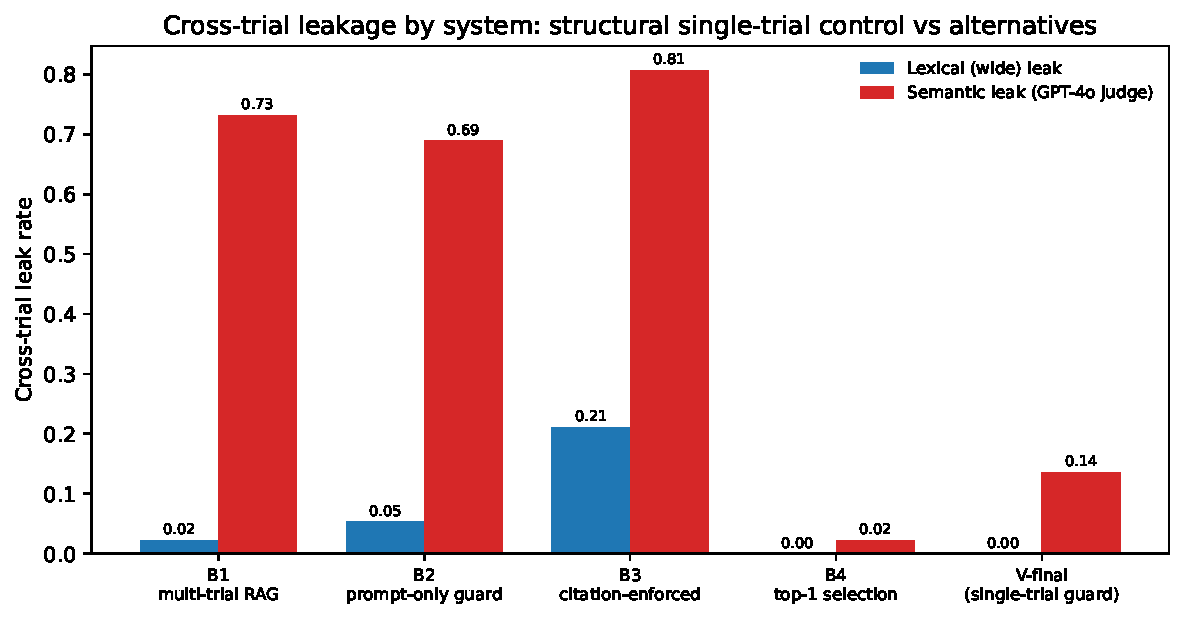
\includegraphics[width=0.9\linewidth]{figures/phase5_baseline_leak_bars.pdf}
\caption{\textbf{Cross-trial leakage by system.} Lexical (wide) and dual-judge-consensus semantic leak for the four baselines and V-final. Multi-trial RAG, prompt-only guarding, and citation enforcement all leak; structural single-trial control (B4, V-final) closes both channels.}
\label{fig:baseline_leak}
\end{figure}

\subsection{Failure taxonomy and claim-level NLI verification}
\label{sec:results_nli}

We classify every consensus-flagged generation into three mutually exclusive categories (Methods, \S\ref{sec:methods_taxonomy}): T1 cross-trial contamination (supported only by a non-selected pool trial), T2 unsupported clinical completion (supported by no pool trial), and T3 ordinary hallucination. This separates the evidence-layer failure the pipeline targets (T1) from generator-level errors (T2/T3). The taxonomy makes the mechanism explicit (Table~\ref{tab:baselines}; Fig.~\ref{fig:taxonomy}): the multi-trial baselines are T1-dominated ($107$--$125$ flags each), whereas structural top-1 selection has \emph{zero} T1, leaving only two T2 and one T3.

We then implement the claim-level verification step the original design only proposed. A natural-language-inference (NLI) post-processor (DeBERTa-v3-large MNLI) redacts an asserted claim when a non-selected pool trial entails it better than the selected trial ($e_{\mathrm{other}} \ge \tau_{\mathrm{NLI}}$ and $e_{\mathrm{other}} > e_{\mathrm{sel}}$), the operational definition of T1 (Methods, \S\ref{sec:methods_nli}). With the threshold fixed on the development pool alone ($\tau_{\mathrm{NLI}}=0.95$), the verifier redacts $8$ of the $12$ both-judges-consensus semantic leaks---exactly the eight that manual review deemed genuine cross-trial content, correctly retaining the two mixed-attribution errors and two judge over-flags---at a $15.1\%$ per-claim utility cost. This converts Theorem~\ref{thm:safety} boundary (iv) into an evaluated mitigation and is the recommended hardening for the smallest backbone.

\begin{figure}[!htbp]
\centering
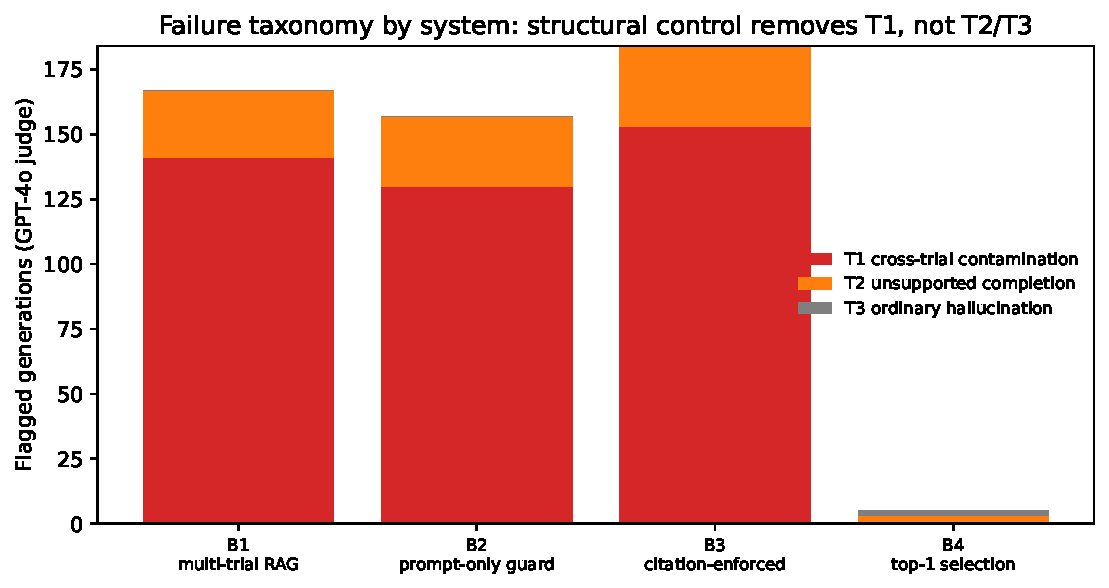
\includegraphics[width=0.78\linewidth]{figures/phase5_taxonomy_breakdown.pdf}
\caption{\textbf{Failure taxonomy by system.} Consensus-flagged generations partitioned into T1 cross-trial contamination, T2 unsupported completion, and T3 ordinary hallucination. Multi-trial baselines are T1-dominated; structural top-1 control removes T1 entirely.}
\label{fig:taxonomy}
\end{figure}

\subsection{Lexical safety is stable across backbones, but fluency is not}
\label{sec:results_backbone_gate}

Lexical leak rate was uniform across the six model families, but parse-ok, commit, and latency varied substantially (Table~\ref{tab:six_backbone}). To examine where the safety behavior arises, we computed Spearman rank correlations between the four continuous selector signals and the per-case judge-pooled rubric scores, stratified by backbone (Supplementary Fig.~S11). For weaker backbones, output quality was more dependent on the strength of the retrieved evidence. Mistral-7B and Llama-3.1-8B showed moderate positive coupling between the raw cross-encoder maximum $\mu$ and factuality (Mistral: $r_s = 0.51$, $p < 0.01$; Llama: $r_s = 0.36$, $p < 0.05$) and between $\mu$ and groundedness (Mistral: $r_s = 0.53$, $p < 0.01$). These models were more factual when the reranker strongly supported the top trial and less reliable when it did not. For Qwen-2.5-7B, signal--rubric correlations were weaker, consistent with a stronger generator operating after the selector had already filtered the evidence. These per-backbone differences in fluency and signal sensitivity did not translate into different lexical leak rates, because the gate ensemble constrained each backbone to the same single-trial evidence pool (Theorem~\ref{thm:safety}).

\subsection{Abstention remains safe and useful when no single trial dominates}
\label{sec:results_abstain}

Real-world onboarding queries frequently fall into the abstain regime, where no single trial dominates the candidate pool. To evaluate this setting, the dual-judge protocol scored all generations on the 82 abstain-regime cases probed with the gate disabled. The narrowing-prompt response, such as ``I could not identify one reliable study; please share the study title or NCT number,'' provides a patient-facing clarification pathway when the system declines to commit. The abstain-regime safety score was at or above $4.0/5$ for every backbone, and the overall rubric mean in the abstain regime was comparable to or higher than the accept-regime mean for the three top backbones (Fig.~\ref{fig:abstain}; Supplementary Table~S12). Operationally, abstention functions as a workflow safeguard rather than a failure mode: it asks the patient for the study title or \texttt{NCT} number, improves the evidence basis for the next interaction, and avoids presenting weakly grounded eligibility content that a coordinator would later need to correct.

To quantify the cost of the high abstention rate, we measured how often an abstained case actually had a relevant trial in its candidate pool. Of the 82 abstain-regime cases, only $18$ ($22.0\%$; 95\% CI $13.6$--$32.5\%$) had a relevant trial available, while $64$ ($78.0\%$) had none, meaning abstention was the correct action. The abstention rate is therefore dominated by cases where committing would have been unsafe rather than by discarded opportunities. Across all five systems (Fig.~\ref{fig:frontier}), the structural single-trial systems occupy the low-leakage region, and top-1 selection attains the highest dual-judge-pooled rubric utility among the four baselines ($3.47/5$; vs.\ $2.88$--$3.12$ for the multi-trial baselines; the B4-over-baseline ranking holds under each judge individually) while holding leakage near zero, indicating that structural control is Pareto-favourable rather than a safety--utility trade.

\begin{figure}[!htbp]
\centering
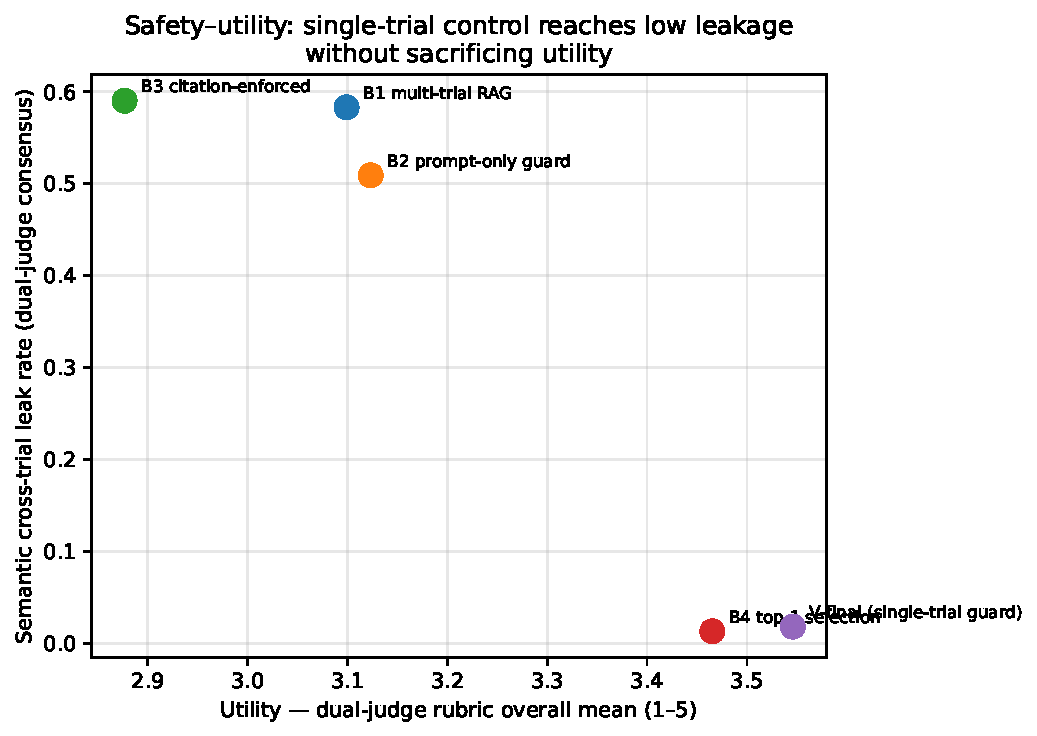
\includegraphics[width=0.78\linewidth]{figures/phase5_safety_utility_frontier.pdf}
\caption{\textbf{Safety--utility trade-off across systems.} $x$-axis: dual-judge-pooled rubric overall mean (baselines pooled over Sonnet~4.5 + GPT-4o; V-final over the full $n=114$ regime). $y$-axis: dual-judge-consensus semantic leak rate. Only the structural single-trial systems (B4, V-final) reach the low-leak region.}
\label{fig:frontier}
\end{figure}

\begin{figure}[!htbp]
\centering
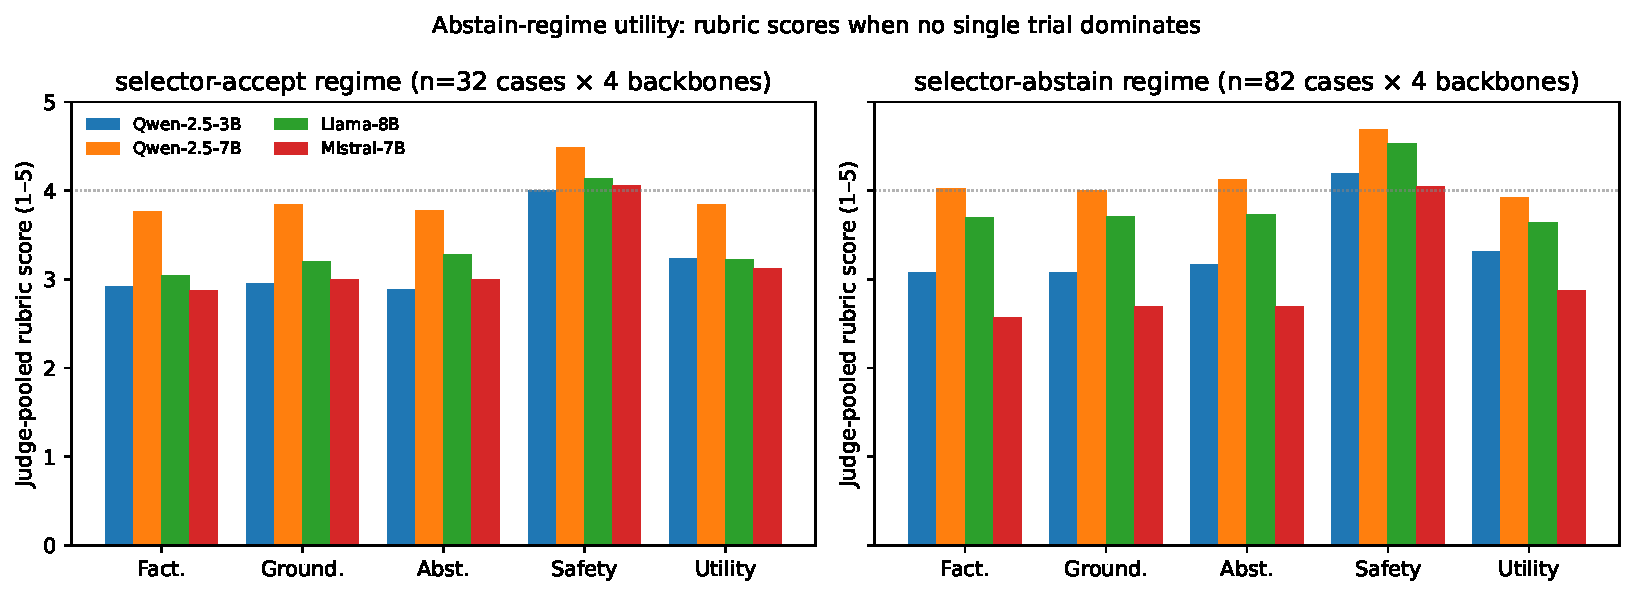
\includegraphics[width=0.96\linewidth]{figures/abstain_regime_quality.pdf}
\caption{\textbf{Abstain-regime utility: judge-pooled rubric scores per regime and backbone.} Safety remains high in both regimes. Overall fluency is comparable or higher in the abstain regime for three of four backbones because the narrowing prompt provides a safe patient-facing clarification pathway under the rubric.}
\label{fig:abstain}
\end{figure}

\subsection{Blind dual-judge evaluation}
\label{sec:results_judge}

Two LLM judges, Claude Sonnet~4.5 and GPT-4o, blind-scored all 684 generations using a five-dimension rubric: factuality, groundedness, abstention appropriateness, safety, and patient utility, each on a 1--5 scale. The blinding protocol is detailed in Methods, \S\ref{sec:methods_judge}. In brief, judges received a SHA1 \texttt{blind\_id}, a per-judge shuffled case order, and normalized JSON output without raw decoder text or model-specific verbose styles. Qwen-2.5-7B achieved the highest overall mean score ($3.95$; 95\% bootstrap confidence interval, $3.76$--$4.14$). The lower-latency Qwen-2.5-3B candidate preserved high safety scores ($4.14$ vs.\ $4.63$ for Qwen-2.5-7B) while reducing mean latency by $44\%$ ($11.0$ vs.\ $19.8$ s). Inter-judge agreement was moderate on substantive dimensions (Spearman $r_s = 0.52$--$0.56$ for factuality, groundedness, and patient utility), ceiling-bound on safety, and more subjective for abstention appropriateness (\S\ref{sec:results_irr_brief}). The full per-backbone rubric table with bootstrap 95\% confidence intervals is reported in Supplementary Table~S11.

\subsection{Inter-judge agreement reflects ceiling effects and abstention subjectivity}
\label{sec:results_irr_brief}

The inter-judge agreement profile reflects two main effects: ceiling saturation on safety and genuine subjectivity in abstention appropriateness. Safety reached a mean score above $4.0$ for every backbone because the gate ensemble drove lexical leak and \texttt{NCT}-hallucination tags to zero. With limited within-unit variance, exact-match agreement was high ($0.32$), but Cohen's $\kappa$ was low ($0.05$), as $\kappa$ is sensitive to prevalence imbalance and reduced score variance \citep{cohen1960kappa,landis1977kappa,gwet2014handbook,hallgren2012irr}. To distinguish ceiling saturation from systematic disagreement, we also examined threshold agreement: the rate at which both judges scored safety $\geq 4$ for the same generation was high across the open-weight cohort (Supplementary Table~S8), indicating agreement on the substantive safety conclusion even where ordinal $\kappa$ was depressed.

Abstention appropriateness showed greater disagreement. Judges differed on what counted as a correctly abstained response, with a mean absolute difference of 2.37 points, reflecting subjectivity in the rule ``commit when evidence is sufficient; abstain otherwise.'' The evidentiary dimensions of factuality, groundedness, and patient utility showed moderate monotonic agreement ($r_s = 0.52$--$0.56$), which is the relevant agreement pattern for the backbone ranking. We also extended pairwise Cohen's $\kappa$ to a three-rater Krippendorff's $\alpha$ analysis on the 15-case ablation pool. On V1, where the rubric retained variance, $\alpha$ ranged from $0.29$ to $0.59$ on substantive dimensions (Supplementary Table~S9). On the guarded variants V2 and V-final, scores were near the rubric ceiling, causing within-unit variance to collapse and $\alpha$ to degenerate. We report this saturation explicitly rather than treating it as evidence of rater instability.

\subsection{Selector score share is not a calibrated triage probability}
\label{sec:results_calib_brief}

The selector's normalized score share $\tau$ is a binary gating signal at a fixed threshold, not a calibrated probability. Tested against three Text REtrieval Conference (TREC)-derived relevance targets on the $n=50$ gold-annotated subset, the Brier Skill Score \citep{brier1950verification} was negative for every target ($-0.10$ for any-match and $-0.45$ for strict; Supplementary Table~S13). A four-feature logistic regression over $(\rho, \tau, \mu, \kappa)$ did not stabilize calibration at $n=50$. These results indicate that $\tau$ should not be used as a per-case triage probability for ranking patients into queues. The gate ensemble is binary, and downstream safety does not depend on probabilistic calibration of $\tau$. Post-hoc temperature scaling \citep{guo2017calibration} or Platt scaling \citep{platt1999probabilistic} on a larger gold pool would be required before using selector scores probabilistically.


% ============================================================

\section{Discussion}
\label{sec:discussion}

\paragraph{Cross-trial conflation as an evidence-layer target.}
The central design decision in this work is to address cross-trial conflation at the evidence layer rather than relying only on the generator. The five-gate selector ensemble constrains the downstream eligibility, consent-style, and teach-back modules to draw from a single accepted trial. The postprocessor rewrites uncited fields to an explicit fallback string, and the schema maps non-parsing outputs to \emph{cannot-determine}. Together, these mechanisms convert a stochastic generation problem into a structured safety-control problem, which we formalize in Theorem~\ref{thm:safety}. The empirical result of zero lexical leakage across 684 generations from six model families, together with the per-gate ablation showing that no single gate alone explains the result (Table~\ref{tab:per_gate}), indicates that lexical safety arises from the guard ensemble and postprocessor rather than from a specific generator backbone.

\paragraph{Conditional sufficiency with explicit boundary conditions.}
\begin{theorem}[Conditional sufficiency for zero lexical leakage under schema-constrained outputs]
\label{thm:safety}
Let $L \in \{0, 1\}$ denote a lexical cross-trial leak event under either operational definition in Methods, \S\ref{sec:methods_leak_def}. If conditions {\rm(C1) single-trial evidence}, {\rm(C2) bounded fallback}, and {\rm(C3) schema enforcement} all hold for a generation, and the parametric-memory channel emits no non-$t^\star$ trial identifier or distinctive non-selected-trial vocabulary at audit time, then $L = 0$.
\end{theorem}

\begin{proof}[Proof sketch]
A lexical leak requires a non-selected trial identifier or distinctive non-selected-trial vocabulary to appear in a model-emitted text field. By (C1), the only trial evidence passed to the generator is from the selected trial $t^\star$. By (C2), every consent field that lacks a cited passage in $\mathcal{E}^\star$ is rewritten to an explicit fallback string by the postprocessor, which prevents uncited consent explanations from introducing non-selected-trial content. By (C3), non-parsing eligibility outputs collapse to \emph{cannot-determine}, which prevents narrative drift from entering the rendered eligibility output. The remaining channel is direct generation of non-$t^\star$ content from parametric memory. We instrument this channel with three detectors: a narrow \texttt{NCT}-identifier detector, a wide entity-resolved token detector, and a semantic LLM-judge detector. The two lexical detectors identify $0/684$ leaks, while the semantic detector identifies $12/684$ generations ($1.75\%$) under both-judges-agree consensus. Thus, the schema-constrained lexical channels are closed by construction under (C1)--(C3), while the residual paraphrased semantic channel is empirically bounded rather than eliminated.
\end{proof}

This sufficiency claim is conditional and has explicit boundary conditions. The lexical bound may fail if: (i) prompts pass unvalidated raw multi-trial context to the generator; (ii) a backbone emits text outside the schema and the postprocessor fails to recover a safe fallback; (iii) corpus updates introduce new trials with overlapping distinctive vocabulary and the wide-leak vocabulary is not recomputed; or (iv) the model generates paraphrased cross-trial content that contains neither a non-selected \texttt{NCT} identifier nor distinctive non-selected-trial vocabulary. The fourth case is the residual semantic channel measured by the LLM-judge detector. In our audit, this channel appears in $12/684$ generations under both-judges-agree consensus and is concentrated in structurally adversarial cases (\S\ref{sec:results_adversarial}). We implement and evaluate a claim-level NLI verification step for this channel (\S\ref{sec:results_nli}): it redacts $8$ of the $12$ consensus leaks---exactly those manual review deems genuine cross-trial content---at a $15.1\%$ per-claim utility cost, converting this boundary condition from a proposed mitigation into an evaluated one.

\paragraph{Positioning relative to prior trial-matching systems.}
Existing AI-assisted trial-matching systems and the proposed pipeline target different outputs. DeepEnroll \citep{zhang2020deepenroll}, COMPOSE \citep{gao2020compose}, TrialGPT \citep{jin2024trialgpt}, and PRISM \citep{gupta2024prism} focus primarily on per-(patient, trial) eligibility prediction, ranking, or criterion-level reasoning. In contrast, the proposed pipeline produces a multi-field onboarding bundle that includes an eligibility triage label, supported and missing facts, consent-style explanation, and teach-back prompts. Its design objective is not to improve match accuracy directly, but to enforce single-trial consistency and audit traceability in patient-facing outputs.

Table~\ref{tab:prior_systems} summarizes this difference in design surface. A direct metric-level comparison would require either applying the proposed gate ensemble to each prior system's patient-facing output pipeline or adapting those systems to generate the same multi-field onboarding bundle under the same evidence constraints. Because these systems were not developed for the same output type, we position the present contribution as complementary to match-accuracy optimization. In principle, the gate ensemble could be layered on top of any retrieval-augmented trial-matching back end that exposes per-trial evidence.

\begin{table}[!htbp]
\centering
\caption{\textbf{Qualitative comparison to prior trial-matching systems.} The systems are not directly comparable on a single metric because they target different output types. The proposed pipeline is complementary to match-accuracy optimization and is designed to enforce single-trial consistency in patient-facing onboarding outputs.}
\label{tab:prior_systems}
\small
\setlength{\tabcolsep}{4pt}
\begin{tabularx}{\linewidth}{l X X X X X}
\toprule
System & Output & Single-trial guard & Patient-facing & Audit JSON & Leak rate reported \\
\midrule
DeepEnroll \citep{zhang2020deepenroll}  & per-(patient, trial) match probability & no & no & no & not reported \\
COMPOSE \citep{gao2020compose}          & per-(patient, trial) match score       & no & no & no & not reported \\
TrialGPT \citep{jin2024trialgpt}        & per-criterion verdict and match output & no & partial & partial & not reported \\
PRISM \citep{gupta2024prism}            & per-(patient, trial) ranking           & no & no & no & not reported \\
\textbf{This work}                       & multi-field onboarding bundle          & \textbf{yes} & \textbf{yes} & \textbf{yes} & \textbf{0\% lexical leakage on 684 generations} \\
\bottomrule
\end{tabularx}
\end{table}

\paragraph{Clinical deployment-evaluation workflow.}
The proposed pipeline is a pre-screening clarification aid, not a substitute for protocol-directed eligibility determination, informed consent \citep{kadam2017informed,sudore2009interventions}, or study-team review. Teach-back, in which patients restate key information in their own words, is a long-established clinical-communication practice for health-literacy-sensitive informed consent \citep{kripalani2008teachback,talevski2020teachback,ho2017teachback,tamariz2013improving,glaser2020interventions}. In the proposed workflow, teach-back acts as a bridge between AI-assisted pre-screening and study-team verification.

Figure~\ref{fig:deployment} maps the workflow across four roles: patient, pipeline, study coordinator, and audit/governance layer. Three boundaries are explicit. First, the eligibility vocabulary is intentionally coarse and does not substitute for criterion-by-criterion verification; the postprocessor demotes over-claimed \emph{likely-match} outputs to \emph{possible-match-insufficient-evidence} before rendering a patient-facing response. Second, the patient-facing summary is rebuilt from validated fields rather than copied from raw generation. Third, the audit JSON, including evidence set, selector thresholds, raw output, and postprocessed output, is retained per query so that any patient-facing claim can be traced to a cited passage or to an explicit fallback string.

Before clinical use, this workflow would require institution-specific institutional review board (IRB) review, an updated consent process for AI-assisted onboarding, an audit-retention policy compatible with local privacy requirements, and an escalation pathway for safety-monitoring regressions. Examples of such regressions include non-zero lexical leak rate, parse-failure rate above a configured threshold, or sustained over-abstention.

\begin{figure}[!htbp]
\centering
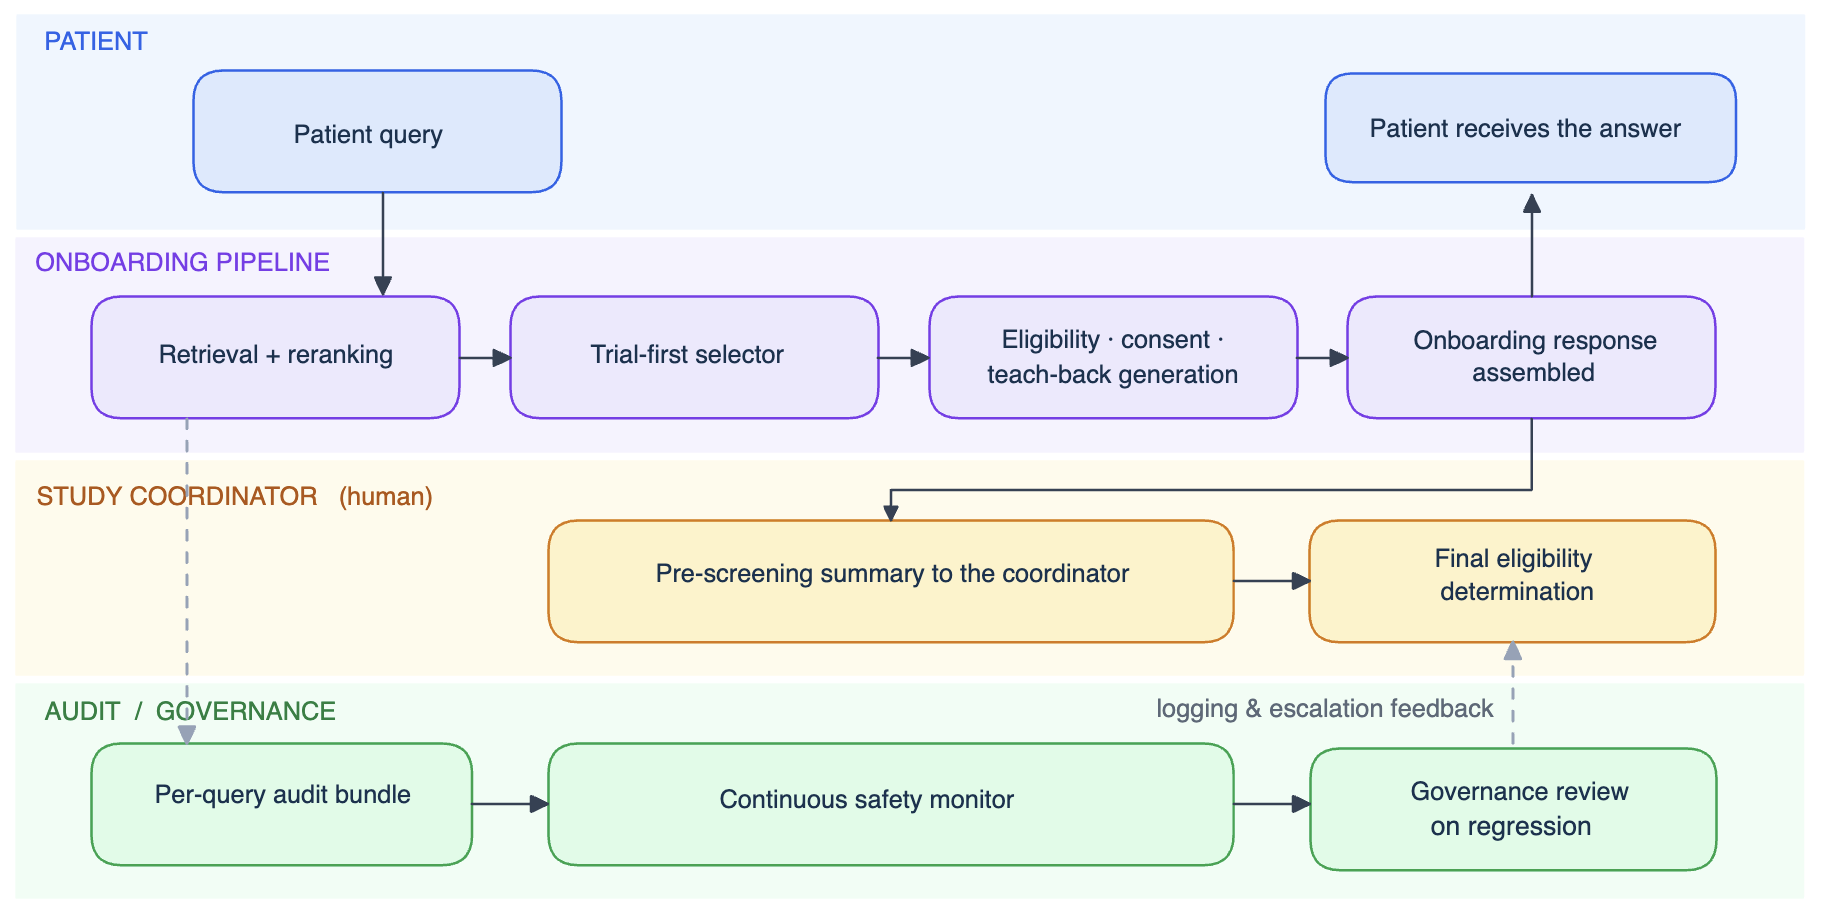
\includegraphics[width=0.96\linewidth]{figures/deployment_workflow.png}
\caption{\textbf{Clinical deployment-evaluation workflow with four roles.} Patient, automated pipeline, study coordinator, and audit/governance layer. The pipeline is a pre-screening clarification aid; the final eligibility decision remains with the study team. Audit JSON is persisted per query. The continuous safety monitor tracks leak, parse-failure, and over-abstention rates and triggers governance review when regression thresholds are crossed.}
\label{fig:deployment}
\end{figure}

\paragraph{Representativeness of the case pool.}
The evaluation pool contains $n=114$ cases from four sources: (i) 50 TREC Clinical Trials topics from the 2021 and 2022 judged pools \citep{roberts2021trec,soboroff2022trec}, (ii) 22 surface-form paraphrases of the curated audit corpus, (iii) 12 hand-crafted vague queries designed to test appropriate refusal to anchor, and (iv) 30 anchor cases spanning seven intent categories: anchor, partial, mismatch, explanation, participation, risk, and consent. The TREC topics provide a recognized information-retrieval benchmark for clinical trial matching, while the curated and paraphrased cases test patient-facing onboarding behaviors that are not captured by standard per-(patient, trial) relevance metrics.

The pool covers two selector regimes, with 32 accept cases and 82 abstain cases, and six therapeutic-area strata: musculoskeletal, cardiovascular, metabolic/endocrine, oncology, neurology/CNS, and Other. We do not claim universal representativeness. No 114-case pool can capture the full diversity of patient language, trial design, institutional workflows, or disease-specific enrollment criteria. Instead, the pool is intended as an auditable stress test for cross-trial consistency across multiple query sources, intent categories, selector regimes, and therapeutic areas. The full provenance manifest is released to support re-stratification and extension by other groups (Supplementary Table~S4).

\paragraph{Limitations.}
This study has six main limitations. \emph{First, the rubric-and-rater design is limited.} The 15-case ablation comparing the unconstrained, strict-abstain, and final guarded variants used a single human auditor. We triangulated this analysis with two independent LLM judges and observed moderate agreement on the V1 stratum where the rubric retained variance, but multi-rater clinician audit remains necessary. The present study should therefore be interpreted as a pre-clinical technical audit of a specific safety failure mode, cross-trial conflation, rather than evidence of patient comprehension or clinical effectiveness.

\emph{Second, the audited regime is finite.} The zero-lexical-leak result is an empirical bound over six model families, six therapeutic areas, two selector regimes, and the evaluated trial corpus, not a universal guarantee. Use in a new institution, new disease area, new backbone family, non-English setting, pediatric population, rare-disease cohort, or other under-represented population \citep{unger2019recruitment,clark2019barriers,fda2022diversity,chang2024fair} would require repeating the leak audit and per-gate ablation on local queries before deployment-oriented evaluation. Fairness audits would also be required for any workflow that incorporates local enrollment records, because healthcare machine-learning systems can reproduce inequities when population structure is not adequately accounted for \citep{obermeyer2019dissecting}.

\emph{Third, clinical utility has not been validated with patients or coordinators.} Utility in this study is assessed using rubric scores rather than patient comprehension, coordinator workload, enrollment outcomes, or consent quality. A prospective human-subject teach-back study is required before making claims about clinical utility.

\emph{Fourth, the selector score share is not calibrated.} The selector score share $\tau$ has a negative Brier Skill Score against held-out relevance targets and should not be used as a per-case triage probability. In patient-facing interfaces, the system should expose only the binary accept/abstain behavior, while using $\tau$ only as an internal monitoring signal.

\emph{Fifth, human evaluation is LLM-judge-based pending independent clinical review.} The headline safety and utility signals rest on two LLM judges; we have prepared a blinded clinical-expert review packet and protocol (Methods, \S\ref{sec:methods_expert}), and recruitment through clinical collaborators is in progress, with independent-reviewer results to be incorporated prior to publication. Until then, these findings should be read as a pre-clinical technical audit. A complementary stronger baseline would also evaluate published trial-matching systems within their own pipelines, which we leave to future work because the output type and available artifacts differ across systems.

\emph{Sixth, the residual semantic channel is reduced but not eliminated.} The claim-level NLI verifier (\S\ref{sec:results_nli}) redacts $8$ of the $12$ both-judges-consensus semantic leaks---the eight that manual review deems genuine cross-trial content---at a $15.1\%$ per-claim utility cost, and is the recommended deployment hardening for the smallest backbone, Qwen-2.5-3B, where the residual concentrates. It does not remove generator-level unsupported-completion errors, and its utility cost argues for selective application (for example, on the adversarial subset with $\rho < 1.5$) rather than globally.



% ============================================================

\section{Methods}
\label{sec:methods}

\subsection{Problem formulation and operational definitions of leakage}
\label{sec:methods_leak_def}

A clinical trial onboarding instance is a tuple $(q, \mathcal{P})$, where $q$ is a patient utterance and $\mathcal{P} = \{p_1, \ldots, p_m\}$ is a set of candidate trial passages. Let $\mathcal{T}$ denote the distinct \texttt{NCT}-indexed trials represented in $\mathcal{P}$. The system produces four structured outputs: (i) an evidence set $E \subseteq \mathcal{P}$; (ii) an eligibility assessment $A = (d, F^+, F^-, R^-)$, where $d$ is one of \emph{likely-match} (LM), \emph{possible-match-insufficient-evidence} (PMIE), \emph{likely-mismatch} (LMM), or \emph{cannot-determine} (CD); (iii) a consent-style explanation $C$, whose fields either cite evidence or default to the fallback string \fallback; and (iv) a teach-back set $T$ of clarification questions conditioned on $F^-$ and $R^-$. A response is defined as leaking when it references a trial other than $t^\star$, the trial accepted by the selector.

We pre-specified three complementary leak detectors. The \emph{narrow lexical detector} flags any \texttt{NCT\textbackslash d\{8\}} regular-expression match other than $t^\star$ in the union of model-emitted text fields after lower-casing and whitespace normalization. The \emph{wide lexical detector} flags either a narrow leak or any token from $\bigcup_{t \neq t^\star} V(t)$, where $V(t)$ is the set of alphabetic title tokens of length at least six that are unique to trial $t$ in the corpus, after removing a curated stop-list of generic clinical English terms; the full stop-list is reported in Supplementary Information \S2.5. The \emph{semantic detector} flags paraphrased factual content, such as an eligibility criterion, dose, schedule, procedure, or sponsor detail, that is supported only by a non-selected trial $t \neq t^\star$ in the retrieval pool. Two independent judges, Claude Sonnet~4.5 and GPT-4o, scored every generation blindly against the selected-trial passages and the top-$k$ non-selected candidate passages. Each judge returned a binary flag, the suspect trial, a claim excerpt of up to 250 characters, and a short rationale. The prompt and per-case audit format are reported in Supplementary Information \S2.6. The primary semantic rate is the conservative both-judges-agree consensus; per-judge marginal rates and the either-judge rate are also reported. The narrow and wide detectors are computed deterministically from persisted JavaScript Object Notation (JSON) outputs, whereas the semantic detector is logged with per-call latency, retry count, and full prompt for reproducibility.

\subsection{Trial-first single-context selector}
\label{sec:methods_selector}

The selector accepts a single dominant trial only if four numerical signals clear deployment thresholds and a generic-question heuristic does not fire. For each distinct trial $t$, we compute a trial-level score
\[
S(t) = \sum_{p \in \mathcal{E},\, \mathrm{doc}(p)=t} \sigma(s(p)),
\]
where $s(p)$ is the cross-encoder score and $\sigma$ is a clipped softplus. Let $t^\star = \arg\max_t S(t)$ denote the top-ranked trial, and let $t^{(2)}$ denote the runner-up. We compute four selector signals: dominance ratio $\rho = S(t^\star)/\max(S(t^{(2)}), \epsilon)$; trial-score share $\tau = S(t^\star)/\sum_t S(t)$; raw maximum cross-encoder score $\mu = \max_{p:\mathrm{doc}(p)=t^\star} s(p)$; and best rank $\kappa$. The context is accepted if and only if $\rho \ge \rho_{\min}$, $\tau \ge \tau_{\min}$, $\mu \ge \mu_{\min}$, $\kappa \le \kappa_{\max}$, and the generic-question flag $g$ does not fire.

The deployed thresholds were $(\rho_{\min}, \tau_{\min}, \mu_{\min}, \kappa_{\max}) = (1.35, 0.28, -4.5, 2)$, with $k_{\text{keep}}=6$ accepted passages. The negative value of $\mu_{\min}$ reflects that $s(p)$ is a raw pre-sigmoid cross-encoder logit and can take any real value; the threshold of $-4.5$ excludes the lowest-confidence reranker outputs while retaining moderately ranked but plausible top passages. The generic-question flag is a deterministic 21-phrase substring detector, validated at precision 0.75 and recall 0.86 on the 15-case audit pool. The full trigger list is reported in Supplementary Table~S3. Pseudocode for the selector and the downstream guarded eligibility, strict consent-style explanation, and teach-back modules is provided in Supplementary Information \S2.

\subsection{Case-set construction and representativeness}
\label{sec:methods_cases}

The $n=114$ evaluation pool combines a curated 30-case audit corpus with an 84-case extension. The curated corpus represents the selector-accept regime and spans seven patient-facing intent categories: anchor, partial, mismatch, explanation, participation, risk, and consent. The extension includes: (i) 50 Text Retrieval Conference (TREC) Clinical Trials 2021 and 2022 topic identifiers, drawn stratified across therapeutic area and topic length and minimally rewritten from third-person clinical sketches into first-person patient-facing questions; (ii) 22 surface-form paraphrases of curated cases; and (iii) 12 hand-crafted vague queries, such as ``I had some bone problems,'' that the deployed system should refuse to anchor.

Each case includes a gold \texttt{NCT} identifier where applicable, an intent category, and a therapeutic-area label assigned by an LLM and manually spot-checked. The area distribution was 14 musculoskeletal/bone, 8 cardiovascular, 19 metabolic/endocrine, 16 oncology, 13 neurology/CNS, and 44 Other. Cases with no clearly dominant trial in the candidate pool were tagged as selector-abstain expected, whereas cases with a clear dominant trial were tagged as selector-accept expected. The deployed thresholds matched the expected behavior for approximately 78\% of cases; disagreements were dominated by conservative abstention on borderline accept cases. The linkage between the 15-case ablation pool used for qualitative design and the $n=114$ safety pool used for the headline audit is documented in Supplementary Information \S2.8. Both case sets are released.

\subsection{Per-gate counterfactual ablation}
\label{sec:methods_pergate}

For each gate $X \in \{\rho, \tau, \mu, \kappa, \mathrm{generic}\}$, we defined a variant \emph{V-final-no-}$X$ that dropped gate $X$ while keeping the other gates active. Because the broader 84-case extension was generated with the gate disabled, leak, commit, and abstain rates for each variant-by-backbone combination were computed from existing JSON records without additional inference. The full per-variant accepted-case lists are released as Supplementary Data.

\subsection{Baseline configurations}
\label{sec:methods_baselines}

Four baselines were pre-registered in a frozen configuration (committed before any baseline generation) and run on the two deployment backbones over the same $n=114$ pool, holding retrieval, the JSON-schema prompt, and the post-processor identical to V-final and varying only the evidence-control mechanism. \textbf{B1} (multi-trial RAG) passes the top-6 reranked passages across all pool trials with no single-trial guard. \textbf{B2} (prompt-only guard) adds a strong anti-mixing instruction (identify the single most relevant trial and answer only from it; otherwise ask for the study title or \texttt{NCT} number). \textbf{B3} (citation-enforced) requires passage-identifier citations for every narrative field and drops uncited fields to the fallback string. \textbf{B4} (top-1 selection) accepts the trial owning the rank-1 passage unconditionally, bypassing the five-gate ensemble while retaining the downstream guarded modules. For B1--B3 the reference trial for the leak detectors is the rank-1 passage's trial. All 912 baseline generations were audited by the same narrow, wide, and dual-judge semantic detectors and scored on the five-dimension rubric.

\subsection{Failure taxonomy}
\label{sec:methods_taxonomy}

Every consensus-flagged generation was classified into three mutually exclusive categories: \textbf{T1} cross-trial contamination (the claim is supported only by a non-selected pool trial), \textbf{T2} unsupported clinical completion (plausible protocol content supported by no pool trial), and \textbf{T3} ordinary hallucination (false or incoherent, not attributable to any trial). The semantic-judge prompt returns a taxonomy label alongside the binary leak flag, and the consensus-flagged cases were adjudicated by the first author. T1 is the evidence-layer failure the pipeline targets; T2 and T3 are generator-level errors that single-trial control is not expected to remove.

\subsection{Claim-level NLI verification}
\label{sec:methods_nli}

The claim-level verifier scores each asserted patient-facing claim with a natural-language-inference model (\texttt{DeBERTa-v3-large-mnli-fever-anli-ling-wanli}), computing the maximum entailment by the selected trial's passages ($e_{\mathrm{sel}}$) and by any non-selected pool trial's passages ($e_{\mathrm{other}}$). A claim is redacted iff $e_{\mathrm{other}} \ge \tau_{\mathrm{NLI}}$ and $e_{\mathrm{other}} > e_{\mathrm{sel}}$---the operational definition of T1 cross-trial contamination---so single-trial-evidence outputs are never modified. The threshold was calibrated on the 15-case development pool alone (highest $\tau_{\mathrm{NLI}}$ with development benign-drop $\le 10\%$; $\tau_{\mathrm{NLI}}=0.95$) before any application to the audit pool, and the frozen verifier was reapplied to all 684 deployed and 912 baseline generations.

\subsection{Independent clinical-expert review protocol}
\label{sec:methods_expert}

To complement the LLM-judge evaluation, we prepared a blinded expert-review packet of 30 generations stratified across selector regime, semantic-flag status, and backbone, including the deployed pipeline and two contrast baselines (B1, B4). Each de-identified dossier presents the patient question, the trial passages shown to the system, and the full patient-facing response under a randomized blinded identifier. Reviewers score each case on the five-dimension rubric plus a binary cross-trial-leak judgment and a T1/T2/T3 label. All queries are synthetic; the packet and scoring instrument are released. Reviewer recruitment through clinical collaborators is in progress, and independent-review results will be incorporated prior to publication.

\subsection{Blind dual-judge evaluation and blinding mechanics}
\label{sec:methods_judge}

Two LLM judges, Claude Sonnet~4.5 and GPT-4o, blind-scored each generation on five integer dimensions: factuality, groundedness, abstention appropriateness, safety, and patient utility, each on a 1--5 scale. Blinding was implemented at the case-by-backbone level. Each pair was assigned a stable identifier,
\[
\texttt{blind\_id} = \mathrm{SHA1}(\texttt{phase3:case\_id:backbone})[:12],
\]
which was the only identifier shown to the judges. The prompt referred to the output as the \emph{assistant response}, without naming the model. Case order was independently shuffled for each judge using different random seeds. Judges received the postprocessed schema-validated JSON output rather than raw decoder text, reducing the risk that model-specific verbosity or formatting would reveal the generator backbone. We also stripped any backbone-name occurrence from the served context and re-served any case in which a parse-extracted field exactly matched a known backbone name.

Per-dimension Cohen's $\kappa$ \citep{cohen1960kappa,landis1977kappa} with linear and quadratic weights, two-way random intraclass correlation coefficient ICC(2,1), Spearman rank correlation $r_s$, exact-match rate, and mean absolute difference are reported in Supplementary Table~S8. Krippendorff's $\alpha$ at the interval level \citep{krippendorff2018content,hayes2007krippendorff} for the three-rater audit, consisting of Human, Claude Sonnet~4.5, and GPT-4o ratings, is reported in Supplementary Table~S9.

\subsection{Retrieval, generation backbones, and audit artifacts}
\label{sec:methods_misc}

Retrieval used a two-stage pipeline: BM25 full-text retrieval followed by cross-encoder reranking on the TREC Clinical Trials 2021 corpus \citep{roberts2021trec,robertson2009bm25,nogueira2019passage,hofstatter2021crossenc,lin2021pyserini}. Dense alternatives based on Sentence-BERT \citep{reimers2019sbert} and contrastive contriever pretraining \citep{izacard2022contriever}, together with BEIR-style zero-shot retrieval evaluation \citep{thakur2021beir}, were considered as fallbacks but did not improve the safety metrics on this corpus (Supplementary Table~S14). The four open-weight backbones were Qwen-2.5-3B-Instruct, Qwen-2.5-7B-Instruct, Meta-Llama-3.1-8B-Instruct, and Mistral-7B-Instruct-v0.3 \citep{qwen25_2024,touvron2023llama2}. The two zero-shot closed-API baselines were GPT-4o, run with \texttt{temperature=0.0} and \texttt{max\_tokens=1500}, and Claude Sonnet~4.5. All six models used the same retrieval, reranker, selector, postprocessor, and prompt; only the generator backbone changed.

Every patient-facing response is accompanied by audit artifacts: (i) reranked evidence with cross-encoder scores; (ii) the trial-level score table; (iii) the context-selector decision with thresholds; (iv) raw model outputs; and (v) postprocessed JSON. These artifacts are persisted per query for downstream review. Retrieval comparison details, including Recall@10, Recall@20, Recall@100, normalized discounted cumulative gain (nDCG)@10 and nDCG@20 across BM25, dense MiniLM, dense BGE-base, reciprocal rank fusion, and the two-stage configuration, are reported in Supplementary Table~S14 and Supplementary Fig.~S13.

% ============================================================
\bmhead{Data availability}
\sloppy
Retrieval experiments used publicly available TREC Clinical Trials 2021 and 2022 data \citep{roberts2021trec,koopman2016trec,soboroff2022trec} and the public ClinicalTrials.gov trial corpus. No patient-identifiable data were collected, processed, or released, and all patient-facing case texts are synthetic. The complete audit bundle generated and analyzed during the current study, including per-case evidence CSV files, selector status JSON files, trial-level scores, raw and postprocessed model outputs, blinded judge JSON-Lines files, per-case and per-backbone rubric scores, the $n=114$ case manifest with provenance tags, per-gate ablation acceptance lists, calibration per-bin tables, and three-way agreement derivations, is publicly available in the project repository at \url{https://github.com/zabirul-islam/clinical-trial-onboarding}. The repository will be archived at Zenodo upon acceptance, and the persistent DOI will be added to the final version. The 660\,MB trial-passage corpus derived from public ClinicalTrials.gov and TREC Clinical Trials 2021/2022 data is mirrored as a HuggingFace dataset at \url{https://huggingface.co/datasets/zabir1996/clinical-trial-onboarding-corpus}. Supplementary Information files included with this article contain the case-manifest summary and the inter-rater agreement tables required to interpret the headline results.
\fussy

\bmhead{Code availability}
The code used for retrieval, reranking, the trial-first selector ensemble, guarded eligibility triage, consent-style explanation, teach-back generation, postprocessing, dual-judge evaluation, inter-rater reliability analysis, per-gate ablation, calibration analysis, and figure generation is released under the MIT license at \url{https://github.com/zabirul-islam/clinical-trial-onboarding}. The repository will be archived at Zenodo upon acceptance, and the DOI will be added to the final version. The pipeline is local-first and can run on commodity GPU hardware; the low-latency candidate backbone, Qwen-2.5-3B-Instruct, fits in less than 8 GB of GPU memory.

\bmhead{Reproducibility statement}
Every numerical claim in the paper is recoverable from the released artifacts. The selector-signal cache, per-case and per-backbone generation JSON files, and dual-judge JSON-Lines files are persisted with stable identifiers. Re-running the figure scripts on these inputs reproduces the deterministic figures exactly and the bootstrapped figures within resampling variability. Re-generation of raw model outputs is non-deterministic for the closed-API backbones, GPT-4o and Claude Sonnet~4.5; therefore, the frozen audit bundle is the canonical reference for reported results.

\bmhead{Competing interests}
The authors declare no financial or non-financial competing interests.

\bmhead{Ethics}
This study used only publicly available trial documents and synthetic patient-facing queries. No human participants were recruited or enrolled, and no patient-identifiable data were collected, processed, or released. The system is not clinically deployed and is positioned as a pre-screening clarification aid rather than a source of eligibility determination or informed consent. In-clinic evaluation or deployment would require institution-specific institutional review board (IRB) review, an updated consent process for AI-assisted onboarding, study-team validation, and governance procedures before any patient-facing use.

\bmhead{Author contributions}
M.Z.I. conceived the study; designed and implemented the retrieval, selector, eligibility, consent-style explanation, and teach-back pipeline; ran all experiments; conducted the per-gate ablation and dual-judge audit; performed the inter-rater reliability and calibration analyses; generated the figures and tables; and drafted the manuscript. G.W. supervised the project, advised on clinical-safety framing and reporting standards, and critically revised the manuscript. All authors read and approved the final manuscript.

\bmhead{Acknowledgements}
This research received no specific grant from any funding agency in the public, commercial, or not-for-profit sectors. Computational resources were provided by institutional resources of Rensselaer Polytechnic Institute. The authors thank colleagues at Rensselaer Polytechnic Institute for helpful discussions on clinical deployment, audit traceability, and patient-facing language.



% ============================================================
\bibliographystyle{unsrtnat}

\bibliography{references}

\end{document}
